\documentclass[11pt]{article}

\usepackage{thumbpdf, amssymb, amsmath, amsthm, microtype,
	    graphicx, verbatim, listings, color, fancybox}
\usepackage[pdftex]{hyperref}
%\usepackage[margin=1in]{geometry}
\usepackage{cawsty}
\usepackage{fullpage}
\usepackage{pseudocode}

\newcommand{\field}[1]{\mathbb{#1}} %requires amsfonts

%\setlength{\parindent}{0pt}

\linespread{1.2}

\begin{document}
\cawtitle{4040-849 Optimization Methods}{Programming Assignment 1 Report}

\begin{problem}{1}
\end{problem}
\begin{solution}

\end{solution}
Solving the optimization problem using the \emph{fmincon} function with the interior-point algorithm yielded the following data for each iteration.

\begin{center}
\includegraphics[scale=0.75]{problem1/problem1.eps}
\end{center}

The values of the objective function and design variables at each iteration are shown in Table \ref{Table1}. In addition, the final values of the objective function, design variables, and constraints after convergence of the interior-point algorithm are shown in the Table \ref{Table2}. From these tables, we can see that the optimal value of the function is $51.8983$, which is obtained when $X^T = [0.0869, 0.6598, 1.8950, -1.4445]$.

\begin{table*}[htbp]
	\centering
    \begin{tabular}{|l|l|l|l|l|l|}
        \hline
        Iteration & Function Value & X1 & X2 & X3 & X4\\ \hline
0 & 100 & 0   &      0    &     0  &  1.0e-07 * 0.1490\\ 
1 & 38.56622 & 0.5758   & 0.8903  &  3.2829  & -0.9824\\ 
2 & 27.67708 & 0.2329   & 1.1938  &  3.2614  & -2.1305\\ 
3 & 46.30828 & 0.0242    &0.1565  &  2.2417  & -1.7951\\ 
4 & 45.35767& 0.3914  &  0.5560  &  2.0194  & -1.8260\\ 
5 & 47.97002 & 0.2306  &  0.6055  &  2.0312  & -1.6103 \\ 
6 & 51.88175 & 0.1067  &  0.6481  &  1.8819  & -1.4587\\ 
7 & 51.92273 & 0.0782  &  0.6694  &  1.9020  & -1.4333 \\ 
8 & 51.89738 & 0.0865  &  0.6589  &  1.8953  & -1.4447 \\
9 & 51.89867 & 0.0871  &  0.6601  &  1.8948  & -1.4445 \\ 
10 & 51.89868 & 0.0869  &  0.6598  &  1.8950  & -1.4445 \\ 
11 & 51.89828 & 0.0869  &  0.6598  &  1.8950  & -1.4445 \\ 
12 & 51.89828 &  0.0869  &  0.6598  &  1.8950 &  -1.4445\\
        \hline
    \end{tabular}
	\caption{Objective function and design variable values for each iteration during the interior-point algorithm.}
	\label{Table1}
\end{table*}

\begin{table*}[htbp]
	\centering
    \begin{tabular}{|l|l|l|l|l|l|l|l|}
        \hline
	Objective Function & X1 & X2 & X3 & X4 & Constraint 1 & Constraint 2 & Constraint 3 \\ \hline
	51.89828 & 0.0869 & 0.6598 & 1.8950 & -1.4445 & -91.1129 & 0 & 0 \\ 
	\hline
    \end{tabular}
	\caption{Final objective function, design variable, and constraint values after convergence of the interior-point algorithm.}
	\label{Table2}
\end{table*}

\begin{problem}{2-a}
\end{problem}
\begin{solution}

Based on the problem description, we seek to optimize the energy stored within the flywheel based on its design specifications, including the maximum permissable mass ($m = 70$ kg), radius ($r = 0.5$ m), rotational speed ($\omega = 3000$ rpm), stress ($\sigma_{max} = 140 \times 10^5$ Pa), density ($\rho = 8000$ kg/m$^3$), and Poissons ratio ($v = 0.3$). We are given the equation for the energy of the flywheel as follows:
\begin{eqnarray*}
E & = & \frac{1}{2}I\omega^2 \\
& = & \frac{1}{4}mr^2\omega^2
\end{eqnarray*}
Now, treating the flywheel radius $r$ and width $w$ as design variables, we can re-write $E$ in terms of $r$ and $w$ by making the following observations.
\begin{enumerate}
	\item $E$ is directly proportional to $\omega$, so we will be able to store the maximum energy only when $\omega$ is at its maximum value (that is, $3000$ rpm = $3000\frac{\text{rev}}{\text{min}}(\frac{1\text{min}}{60\text{s}})(\frac{2\pi \text{rad}}{1 \text{rev}}) = 100\pi$ rad/s).
	\item The mass of the flywheel can be derived using the equation for density ($\rho = \frac{m}{V}$), where the volume $V$ of the flywheel is equal to that of a cylinder with radius $r$ and height $w$ ($V = \pi r^2 w$). Thus, after some algebraic maniupation, we determine the following:
\begin{eqnarray*}
m = \pi r^2 w \rho
\end{eqnarray*} 
\end{enumerate}
Now, with these two observations, we can treat $\omega$ at its maximal value of $100\pi$ rad/s and substitute $m$ with the expression $m = \pi r^2 w \rho$, since $\rho = 8000$ kg/m$^3$ is a fixed value and does not change. Doing this substitution yields the following expression for the energy of the flywheel:
\begin{eqnarray*}
E & = & \frac{1}{4}mr^2\omega^2 \\
& = &\frac{1}{4}\pi r^4 w \rho \omega^2 \\
& = & \frac{1}{4}(8000\pi(100\pi)^2r^4 w) 
\end{eqnarray*}
Now that we have identified the objective function that we must optimize, we must establish the constraints on the design variables $r$ and $w$, which are enumerated below:
\begin{enumerate}
	\item From the problem description we are told that $r \leq 0.5$ m.
	\item From the problem description we are told that $m \leq 70$ kg, so replacing $m$ with our previously derived expression $\pi r^2 w \rho$, we know that $\pi r^2 w \rho \leq 70$ kg, where $\rho = 8000$ kg/m$^3$.
	\item Based on the distortion energy theory of failure that is used to derive the maximal tangential and radial stresses, and assuming that each of these stresses are equal ($\sigma_t = \sigma_r = \frac{1}{2}\rho(3 + v)\omega^2r^2$), we know the following:
\begin{eqnarray*}
\sigma_t^2 + \sigma_r^2 - \sigma_t\sigma_r & = & 2\sigma_t^2 - \sigma_t^2 \\
& = & \sigma_t^2 \\
& = & (\frac{1}{2}\rho(3 + v)\omega^2r^2)^2 \\
& \leq & \sigma_{max}^2
\end{eqnarray*}
Again, using the fact that $\sigma_{max} = (140 \times 10^6)^2$ Pa and $\omega = 100\pi$ rad/s in this maximal case (as well as $v = 0.3$, $\rho = 8000$ kg/m$^3$, and $\sigma_{max} = 140 \times 10^6$ Pa), we can conclude the following:
\begin{eqnarray*}
\frac{1}{4}(8000^2(3.3)^2(100\pi)^4r^4) \leq (140 \times 10^6)^2
\end{eqnarray*}
This can be further reduced by taking the square root of both sides of this expression, which yields the following constraint:
\begin{eqnarray*}
\frac{1}{2}(8000(3.3)(100\pi)^2r^2) \leq (140 \times 10^6)
\end{eqnarray*}
\end{enumerate}
Now, realizing that by maximizing the energy we are minimizing the negation of the energy equation, we can write the problem formally as follows. \\

Minimize
\begin{eqnarray*}
E' = -E = -\frac{1}{4}(8000\pi(100\pi)^2r^4 w) 
\end{eqnarray*}
subject to the nonlinear constraints:
\begin{enumerate}
	\item $r - 0.5 \leq 0$
	\item $8000\pi r^2 w  - 70 \leq 0$
	\item $\frac{1}{2}(8000(3.3)(100\pi)^2r^2) - (140 \times 10^6) \leq 0$
\end{enumerate}
\end{solution}

\begin{problem}{2-b}
\end{problem}
\begin{solution}
Solving this optimization problem using the $fmincon$ function with the interior-point algorithm yielded the following data for each iteration.

\begin{center}
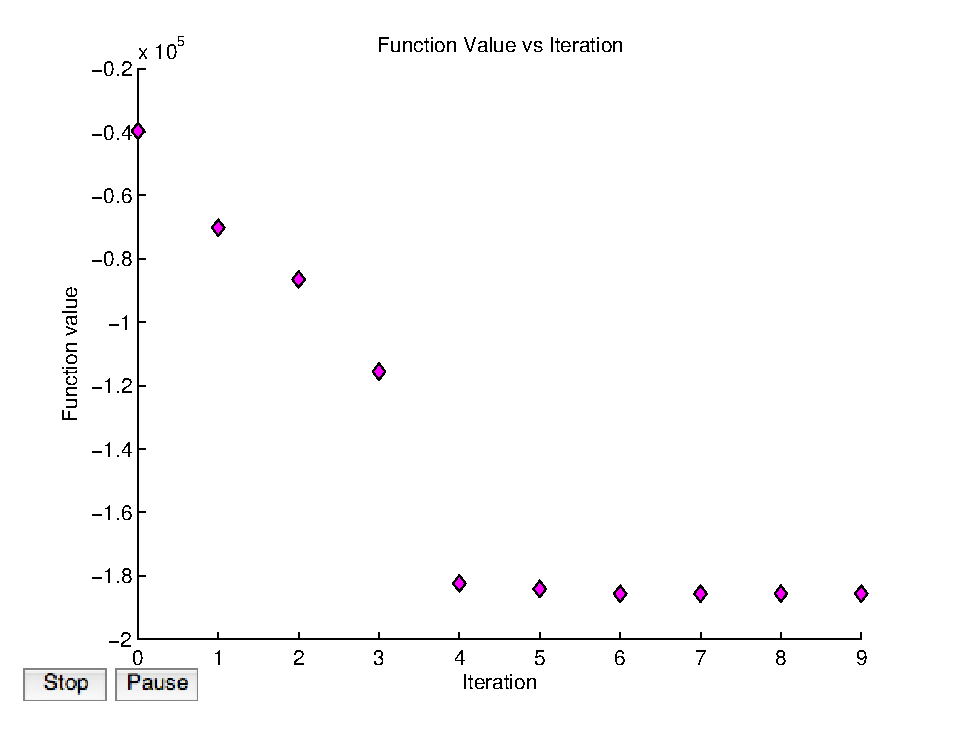
\includegraphics[scale=0.75]{problem2/problem2.eps}
\end{center}

The values of the energy function, radius, and width at each iteration of the interior-point algorithm are shown in Table \ref{Table3}. In addition, the final values of the energy, radius, and width, and constraints after convergence of the interior-point algorithm are shown in the Table \ref{Table4}. It is important to note that since we needed to negate the energy (objective) function to convert it into an appropriate minimization problem for use with the interior-point algorithm, the actual optimal energy value is 185606.1, which is obtained when the radius and width are equal to $0.3278$ m and $0.0259$ m, respectively. 

\begin{table*}[htbp]
	\centering
    \begin{tabular}{|l|l|l|l|}
        \hline
       Iteration & Function Value & Radius & Width\\ \hline
0 & -39688.03	  & 0.2000   & 0.0400\\ 
1 &-70199.91	& 0.2013    & 0.0690 \\ 
2 & -86560.43	& 0.2406 &   0.0417\\ 
3 & -113121.7 & 	0.3155   & 0.0184\\ 
4 & -183952.3	& 0.3252  &  0.0265\\ 
5 & -185019.4	 & 0.3267  &  0.0262\\ 
6 & -185671.7	& 0.3278  &  0.0259\\ 
7 & -185606.9	& 0.3278   & 0.0259\\ 
8 & -185606.1	& 0.3278   & 0.0259\\ 
        \hline
    \end{tabular}
	\caption{Objective function and design variable values for each iteration during the interior-point algorithm.}
	\label{Table3}
\end{table*}

\begin{table*}[htbp]
	\centering
    \begin{tabular}{|l|l|l|l|l|l|}
        \hline
	Objective Function & Radius & Width & Constraint 1 & Constraint 2 & Constraint 3 \\ \hline
	-185606.1 & 0.3278 & 0.0259 & -0.1722 & 0 & -0.7586 \\ 
	\hline
    \end{tabular}
	\caption{Final objective function, design variable, and constraint values after convergence of the interior-point algorithm.}
	\label{Table4}
\end{table*}

\end{solution}

\end{document}
